\documentclass{beamer}
\usepackage{../../shared/styles/custom}
\usepackage{../../shared/styles/conventions}

\newcommand{\vecuvec}[2] %start point, end point (of vector)
{   \VECTORSUB(#2)(#1)(\sola,\solb,\solc)
	\UNITVECTOR(\sola, \solb, \solc)(\sola,\solb,\solc)
	%arrow in blue
	\draw[->,thick,blue] (#1) -- (#2); 
	%corresponding unit-vector in red:
	\edef\temp{\noexpand\draw[->, thick,red] (#1) -- ($(#1)+(\sola,\solb,\solc)$);}
	\temp
}

%\beamerdefaultoverlayspecification{<+->}

\title{Linear Regression}
\date{\today}
\author{Nipun Batra and the teaching staff}
\institute{IIT Gandhinagar}
\begin{document}
\maketitle

\begin{frame}\begin{tcolorbox}
		$weight_{i} \approx \theta_{0} + \theta_{1} \cdot height_{i}$
	\end{tcolorbox}
\end{center}
\end{frame}

\begin{frame}\[\yhat_{n \times 1} = \mX_{n \times d} \vtheta_{d \times 1} \]

%W(N \times 1); X(N\times 2); \theta(2 \times 1);

\pause \begin{itemize}
    \item<+-> $\theta_{0}$ - Bias Term/Intercept Term
    \item<+-> $\theta_{1}$ - Slope
\end{itemize}
\end{frame}

\begin{frame}Examples in multiple dimensions.\\
\pause One example is to predict the water demand of the IITGN campus

\small{
\begin{center}
  \pause  \begin{tcolorbox}
        Demand = f(\# occupants, Temperature)
    \end{tcolorbox}
\end{center}

\begin{center}
    \pause \begin{tcolorbox}
        Demand = Base Demand + $K_{1}$ * \# occupants + $K_{2}$ * Temperature
    \end{tcolorbox}
\end{center}
}

\end{frame}

\begin{frame}\[\begin{bmatrix}
        \hat{y_{1}}\\
        \hat{y_{2}} \\
        \vdots \\
        \hat{y_{N}}
    \end{bmatrix}_{N \times 1}
    =     \begin{bmatrix}
        1 & x_{1,1} & x_{1,2} & \dots & x_{1,M}\\
        1 & x_{2,1} & x_{2,2} & \dots & x_{2,M}\\
        \vdots & \vdots & \vdots & \dots & \vdots\\
        1 & x_{N,1} & x_{N,2} & \dots & x_{N,M}\\
        % y_{2} \\
        % \vdots \\
        % y_{N}
    \end{bmatrix}_{N \times (M+1)}
    \begin{bmatrix}
        \theta_{0}\\
        \theta_{1}\\
        \vdots \\
        \theta_{M}\\
    \end{bmatrix}_{(M+1)\times 1}
   \]
   
%   \begin{center}
%       \textbf{Y}: N\times1; \textbf{X}: N\times(M+1); $\mathbf{\theta}$: (M+1)\times1 
%   \end{center}
   
  \pause  \begin{tcolorbox}
   \begin{center}

   $ \hat{Y} = X\theta$
   \end{center}
   \end{tcolorbox}

\end{frame}

\begin{frame}\begin{tcolorbox}
       $ Y = X\theta + \epsilon$
    \end{tcolorbox}
    
    \pause To Learn: $\theta$ \\
    \pause Objective: ${\text{minimize }} \epsilon_{1}^2 + \epsilon_{2}^2 + \dots + \epsilon_{N}^2$  
\end{frame}

\begin{frame}Objective:   Minimize $\epsilon^{T}\epsilon$    
\end{center}
\end{frame}

\begin{frame}The above table represents the data after transformation \\
\pause Now, we can write $\hat{s}=f(t, t^2)$ \\
\pause Other transformations: $\log(x), x_1\times x_2$
\end{frame}

\begin{frame}\\A linear combination of $\vv_{1},\vv_{2},\vv_{3},\dots,\vv_{i}$ is of the following form
    
    \pause \begin{equation*}
        \alpha_{1}\vv_{1}+			\alpha_{2}\vv_{2}+			\alpha_{3}\vv_{3}+
        \dots+\alpha_{i}\vv_{i}
    \end{equation*}
    
    where $\alpha_{1},\alpha_{2},\alpha_{3},\dots,\alpha_{i} \in \Real$
    
\end{frame}

\begin{frame}The span of  $v_{1},v_{2},\dots,v_{i}$ is denoted by SPAN\{$v_{1},v_{2},\dots,v_{i} $\}
    
    \pause \begin{equation*}
    \{	\alpha_{1}v_{1}+			\alpha_{2}v_{2}+
    \dots+\alpha_{i}v_{i} \hspace{1em}\vert \hspace{1em}  \alpha_{1},\alpha_{2},\dots,\alpha_{i} \in {\rm I\!R}\}
    \end{equation*}
    
    \pause  It is the set of all vectors that can be generated by linear combinations of $v_{1},v_{2},\dots,v_{i}$.

    \pause If we stack the vectors $v_{1},v_{2},\dots,v_{i}$ as columns of a matrix $V$, then the span of $v_{1},v_{2},\dots,v_{i}$ is given as $V\alpha$ where $\alpha \in {\rm I\!R}^{i}$
\end{frame}

\begin{frame}Can we obtain a point (x, y) s.t. x = 3y? \\
\pause No \\ 
\pause Span of the above set is along the line y = 2x

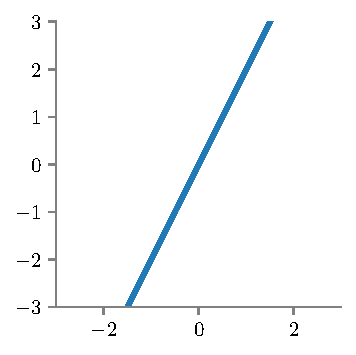
\includegraphics[scale=0.6]{../assets/linear-regression/figures/geoemetric-span-4.pdf}

\end{frame}

\begin{frame}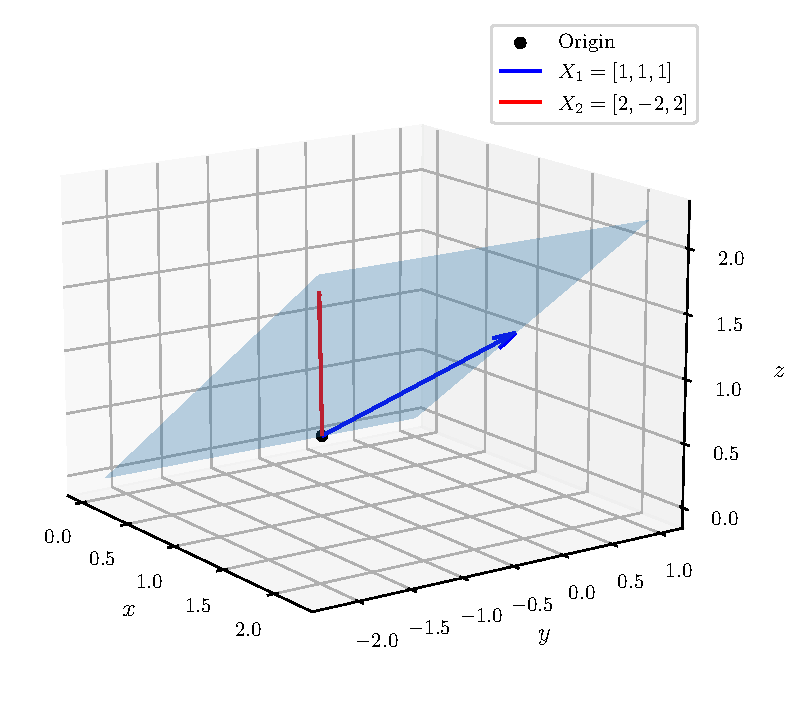
\includegraphics[width=0.6\textwidth]{../assets/linear-regression/figures/geometric-1.pdf}

\pause The span is the plane $z=x$ or $x_3=x_1$
\end{frame}

\begin{frame}This condition arises when the $|X^{T}X|$ = 0.
    
    \begin{equation}
    X = \begin{bmatrix}
    1 & 1& 2\\
    1 & 2& 4\\
    1 & 3& 6\\
    \end{bmatrix}
    \end{equation}
    
    \pause The matrix X is not full rank. 
    \end{frame}

    \begin{frame}\begin{center}
        P = $\theta_{0}$ + $\theta_{1}$*\#Vehicles + $\theta_{1}$*
        \textit{Wind speed} + $\theta_{3}$ * \textit{Wind Direction}
    \end{center}
    
    \pause But, wind direction is a categorical variable. \\
    \pause It is denoted as follows \{N:0, E:1, W:2, S:3 \}\\
    \vspace{3em}
    
    \pause Can we use the direct encoding? \\
    \pause Then this implies that S$>$W$>$E$>$N
    \end{frame}
    
    \begin{frame}The N-1 variable encoding is better because the N variable encoding can cause multi-collinearity. \\
    
    \pause Is it S = 1 - (Is it N + Is it W + Is it E) 
    
    \end{frame}

    \begin{frame}W and S are related by one bit. 
    
    \pause This introduces dependencies between them, and this can cause confusion in classifiers.
    \end{frame}
    
    \begin{frame}Encoding
    
    \begin{center}
    \pause \begin{tabular}{c|c}
    Is Female& height\\
    \hline
    \hline
    1 & \dots \\
    1 & \dots \\
    1 & \dots \\
    0 & \dots \\
    0 & \dots \\
    \end{tabular}
    \end{center}
    
    \end{frame}
    
    \begin{frame}\begin{tabular}{c|c}
            Is Female& height\\
            \hline
            \hline
            1 & 5 \\
            1 & 5.2 \\
            1 & 5.4 \\
            0 & 5.8 \\
            0 & 6 \\
        \end{tabular}
    \end{center}
    \pause $height_{i}$ = $\theta_{0}$ + $\theta_{1}$ *  (Is Female) + $\epsilon_{i}$\\
    \vspace{1em}
    \pause We get $\theta_0$ = 5.9 and $\theta_1$ = -0.7\\
    \pause $\theta_{0}$ = Avg height of Male = 5.9\\
    \pause $\theta_{0} + \theta_{1}$ is chosen based (equal to) on 5, 5.2, 5.4 (for three records). \\
    \pause $\theta_{1}$ is chosen based on 5-5.9, 5.2-5.9, 5.4-5.9
    \pause $\theta_{1}$ = Avg. female height (5+5.2+5.4)/3 - Avg. male height(5.9)
    \end{frame}
    
    \begin{frame}\(x_{i}=\left\{\begin{array}{ll}{1} & {\text { if } i \text { th person is female }} \\ {-1} & {\text { if } i \text { th person is male }}\end{array}\right.\)
    
    \pause \(y_{i}=\theta_{0}+\theta_{1} x_{i}+\epsilon_{i}=\left\{\begin{array}{ll}{\theta_{0}+\theta_{1}+\epsilon_{i}} & {\text { if } i \text { th person is female }} \\ {\theta_{0}-\theta_{1}+\epsilon_{i}} & {\text { if } i \text { th person is male. }}\end{array}\right.\)

    \pause Now, $\theta_{0}$ can be interpreted as average person height. $\theta_{1}$ as the amount that female height is above average and male height is below average.
\end{frame}

\section{Practice and Review}

\begin{frame}\item When does the normal equation have a unique solution?
\pause
\item How do polynomial features help with non-linear relationships?
\pause
\item What are the assumptions behind linear regression?
\end{enumerate}
\end{frame}

\begin{frame}\textbf{Violation Consequences:}
\begin{itemize}
\item Biased coefficient estimates
\item Invalid confidence intervals
\pause
\item Poor prediction performance
\end{itemize}
\end{frame}

\begin{frame}{Key Takeaways}
\begin{itemize}
\item \textbf{Linear Model}: Assumes linear relationship between features and target
\pause
\item \textbf{Least Squares}: Minimizes sum of squared residuals
\pause
\item \textbf{Normal Equation}: Closed-form solution when $\mX\tp\mX$ is invertible
\pause
\item \textbf{Geometric View}: Projection onto column space of design matrix
\pause
\item \textbf{Feature Engineering}: Basis expansion enables non-linear modeling
\pause
\item \textbf{Foundation}: Building block for more complex models
\end{itemize}
\end{frame}

\end{document}
